\renewcommand{\theequation}{\theenumi}
\begin{enumerate}[label=\thesubsection.\arabic*.,ref=\thesubsection.\theenumi]
\numberwithin{equation}{enumi}

\item To find the shortest distance between the lines 
\begin{align}
    L_1\colon \vec{x}=\myvec{1\\2\\1}+\lambda_1\myvec{1\\-1\\1}\label{eq:pseudo:1}\\
    L_2\colon \vec{x}=\myvec{2\\-1\\-1}+\lambda_2\myvec{2\\1\\2}\label{eq:pseudo:2}
\end{align}
\item If the two lines intersect,
\begin{align}
\vec{x}_1 + \lambda_1 \vec{m}_1
=\vec{x}_2 + \lambda_2 \vec{m}_2
\\
\implies \myvec{\vec{m}_1 & \vec{m}_2}\myvec{\lambda_1 \\ -\lambda_2} = \vec{x}_2 - \vec{x}_1
\\
\text{or, } \vec{M}\myvec{\lambda_1 \\ -\lambda_2} = \vec{x}_2 - \vec{x}_1
\label{eq:pseudo_intersect}
\end{align}
%
where 
\begin{align}
\label{eq:pseudo_xm}
\vec{x}_1 = \myvec{1\\2\\1},
\vec{x}_2 = \myvec{2\\-1\\-1},
\vec{m}_1 = \myvec{1\\-1\\1},
\vec{m}_2 = \myvec{2\\1\\2}.
\\
\vec{M} =\myvec{\vec{m}_1 & \vec{m}_2}
\label{eq:pseudo_rect}
\end{align}
\eqref{eq:pseudo_intersect} can be expressed as the matrix equation 
\begin{align}
\myvec{
1 & 2
\\
-1 & 1
\\
1 & 2
}
\vec{x} =
\myvec{1 \\ -3 \\ -2}
\label{eq:pseudo_mat_eq}
\end{align}

From the augmented matrix in \eqref{eq:pseudo_intersect},
%
\begin{align}
%    \myvec{1\\2\\1}+\lambda_1\myvec{1\\-1\\1}=\myvec{2\\-1\\-1}+\lambda_2\myvec{2\\1\\2}\\
%    \lambda_1\myvec{1\\-1\\1}-\lambda_2\myvec{2\\1\\2}=\myvec{1\\-3\\-2}\\
%    \myvec{1 & -2\\-1 & -1\\1 & -2}\myvec{\lambda_1\\\lambda_2}=\myvec{1\\-3\\-2}\\
%    \intertext{The Augmented matrix will be}
    \myvec{1 & -2 & 1\\-1 & -1 & -3\\1 & -2 & -2}\\
    \myvec{1 & -2 & 1\\-1 & -1 & -3\\1 & -2 & -2}\xleftrightarrow{R_1=R_1-R_2}\myvec{0 & 0 & 3\\-1 & -1 & -3\\1 & -2 & -2}
\end{align}
The above matrix has a $rank=3$. Hence the lines do not intersect.
\item Let 
\begin{align}
\vec{A}=\vec{x}_1 + \lambda_1 \vec{m}_1
\\
\vec{B}=\vec{x}_2 + \lambda_2 \vec{m}_2
\label{eq:pseudo_AB}
\end{align}
be the closest points on $L_1$ and $L_2$ respectively.  Then the shortest distance between two skew lines 
will be the length of line perpendicular to both the lines $L_1$,$L_2$ and passing through $A$ and $B$.
Thus, 
\begin{align}
    \vec{m_1}^T\brak{\vec{A}-\vec{B}}=0\label{eq:pseudo:32}\\
    \vec{m_2}^T\brak{\vec{A}-\vec{B}}=0\label{eq:pseudo:34}\\
\implies \vec{M}^T\brak{\vec{A}-\vec{B}} = 0
\label{eq:pseudo:MAB}
\end{align}
From \eqref{eq:pseudo_AB} and \eqref{eq:pseudo_rect}
%
\begin{align}
    \vec{A-B}=\vec{x_1-x_2}+\vec{M}\myvec{\lambda_1\\ -\lambda_2}
\label{eq:pseudo:31}
\end{align}
and using \eqref{eq:pseudo:MAB}, in the above, 

%\begin{align}
%    \vec{m_1^T}(\vec{x_1-x_2})+\vec{m_1^T}(\vec{m_1} & -\vec{m_2})\begin{pmatrix}\lambda_1 \\ \lambda_2\end{pmatrix}=0\label{eq:33}
%\end{align}
%The dot product of $\vec{m_2}$ with the line ${AB}$ is
%\begin{align}
%    \vec{m_2}^T\brak{\vec{A-B}}=0\label{eq:34}\\
%    \vec{m_1^T}(\vec{x_1-x_2})+\vec{m_2^T}(\vec{m_1} & -\vec{m_2})\myvec{\lambda_1 \\ \lambda_2}=0\label{eq:35}
%\end{align}
%Let the matrix $\vec{M}$ be
%\begin{align}
%    \vec{M}=\myvec{\vec{m_1}^T\\\vec{m_2}^T}\label{eq:36}
%\end{align}
%Combining the equations \eqref{eq:33} and \eqref{eq:35} in matrix form,using equation \eqref{eq:36}, we get
\begin{align}
    \vec{M}^T\vec{M}\myvec{\lambda_1\\-\lambda_2} = \vec{M}^T\brak{\vec{x}_2-\vec{x}_1}
\label{eq:pseudo_ls}
\end{align}
%simplifying it further
%\begin{align}
%    \vec{M}\vec{M}^T\begin{pmatrix}\lambda_1\\-\lambda_2\end{pmatrix}=\vec{M}\vec{(x_2-x_1)}
%\end{align}
\item Substituting the values from \eqref{eq:pseudo_xm} in \eqref{eq:pseudo_ls} and forming the augmented matrix,
%To find the points on the lines which make up the shortest distance we need to find $\lambda_1$ and $\lambda_2$ using the above expression to get the augmented form
\begin{align}
%    \myvec{\vec{m_1}^T\vec{m_1} & \vec{m_1}^T\vec{m_2}\\\vec{m_2}^T\vec{m_1} & \vec{m_2}^T\vec{m_2}}\myvec{\lambda_1\\-\lambda_2}=\myvec{\vec{m_1}^T\vec{(x_2-x_1)}\\\vec{m_2}^T\vec{(x_2-x_1)}}\\
%    \myvec{\vec{m_1}^T\vec{m_1} & \vec{m_1}^T\vec{m_2} & \vec{m_1}^T\vec{(x_2-x_1)}\\\vec{m_2}^T\vec{m_1} & \vec{m_2}^T\vec{m_2} & \vec{m_2}^T\vec{(x_2-x_1)}}\\
%    \intertext{we know that}
%    \vec{x_1}=\myvec{1\\2\\1},\vec{x_2}=\myvec{2\\-1\\-1},\vec{m_1}=\myvec{1\\-1\\1} and  \vec{m_2}=\myvec{2\\1\\2}
%    \intertext{so the augmented matrix will be}
    \myvec{3 & 3 &2\\ 3 & 9 & -5}\\
    \myvec{3 & 3 &2\\ 3 & 9 & -5}\xleftrightarrow{R_2=R_2-R_1}\myvec{3 & 3 &2\\ 0 & 6 & -7}\\
    \myvec{3 & 3 &2\\ 0 & 6 & -7}\xleftrightarrow{R_1=2R_1-R_2}\myvec{6 & 0 & 11\\ 0 & 6 & -7}\\
    \myvec{6 & 0 & 11\\ 0 & 6 & -7}\xleftrightarrow{R_1=\frac{R_1}{6},R_2=\frac{R_2}{6}}\myvec{1 & 0 & \frac{11}{6}\\ 0 & 1 & \frac{-7}{6}}\\
    \lambda_1=\frac{11}{6},\lambda_2=\frac{7}{6}
\end{align}
yielding
\begin{align}
A=\frac{1}{6}\myvec{17\\1\\17},
B=\frac{1}{6}\myvec{26\\1\\8}. 
\end{align}
%
\item The distance is then obtained as
%The shortest distance between the lines is the distance between the points $A$ and $B$.
\begin{align}
    \norm{\vec{B}-\vec{A}} 
%    =\norm{\frac{1}{{6}}\myvec{17\\1\\17}-\frac{1}{{6}}\myvec{26\\1\\8}}\\
    =\frac{3}{\sqrt{2}}
\end{align}
%Therefore the shortest distance between the given lines is $\frac{3}{\sqrt{2}}$.\par
%
%The unit vector perpendicular to lines
%\begin{align}
%    Line_1\colon \vec{x}=\vec{x_1}+\lambda_1\vec{m_1}\\
%    Line_2\colon \vec{x}=\vec{x_2}+\lambda_1\vec{m_2}
%\end{align}
%can be found by 
%\begin{align}
%    \vec{n}=\frac{\vec{A-B}}{\norm{\vec{A-B}}}\\
%    \vec{n}=\frac{\frac{1}{{6}}\myvec{17\\1\\17}-\frac{1}{{6}}\myvec{26\\1\\8}}{\frac{3}{\sqrt{2}}}\\
%    \vec{n}=\frac{1}{\sqrt{2}}\begin{pmatrix}-1\\0\\1\end{pmatrix}
%\end{align}
%
%So the unit vector perpendicular to both $L_1$ and $L_2$ is
%\begin{align}
%    \vec{n}=\frac{1}{\sqrt{2}}\begin{pmatrix}-1\\0\\1\end{pmatrix}
%\end{align}
Fig.     \ref{fig:pseudo_Skew_lines} shows the various points and distances between the lines.
\begin{figure}[!ht]
\centering
    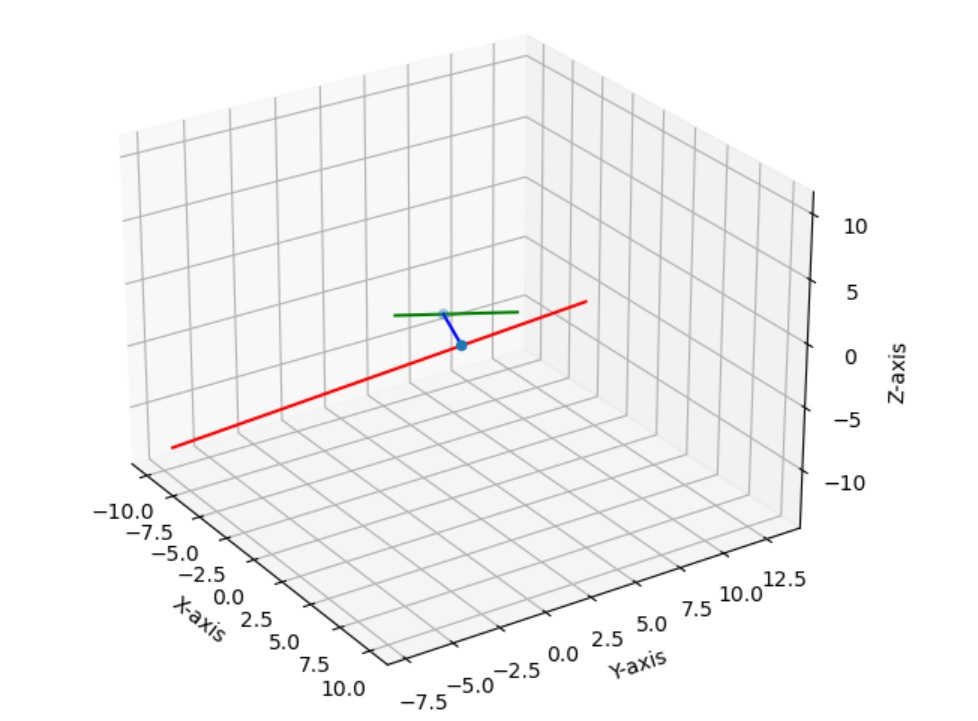
\includegraphics[width=\columnwidth]{./figs/pseudo/assignment2.jpg}
    \caption{This is the plot of the given skew lines and the blue line indicates the normal to the given lines}
    \label{fig:pseudo_Skew_lines}
\end{figure}


\end{enumerate}
